


\section{Data-analysis tips}\label{lab-5-data-analysis-tips}

To give you an idea about the analyses you will be performing, we will
again create simulated data to mimic aspects of the experiment, and then
go through the steps of performing the analysis.

We will simulate data for the switching cost. Specifically, we will
imagine that women have a smaller switching cost than men. The code
below generates sample data for 10 women and 10 men, who each have mean
reactions in the repeat and switch conditions. For women, the mean
reaction times were 580 ms for repeat and 600 ms for switch sequences,
for a total expected switch cost of 20 ms. For men, the mean reaction
times were 580 ms for repeat and 650 ms for switch sequences, for a
total expected switch cost of 70 ms.

\subsection{Simulating the data}\label{simulating-the-data}

\begin{Shaded}
\begin{Highlighting}[]
\NormalTok{women_switch <-}\KeywordTok{round}\NormalTok{(}\KeywordTok{rnorm}\NormalTok{(}\DecValTok{10}\NormalTok{,}\DecValTok{600}\NormalTok{,}\DecValTok{20}\NormalTok{))}
\NormalTok{women_repeat <-}\KeywordTok{round}\NormalTok{(}\KeywordTok{rnorm}\NormalTok{(}\DecValTok{10}\NormalTok{,}\DecValTok{580}\NormalTok{,}\DecValTok{20}\NormalTok{))}
\NormalTok{men_switch <-}\KeywordTok{round}\NormalTok{(}\KeywordTok{rnorm}\NormalTok{(}\DecValTok{10}\NormalTok{,}\DecValTok{650}\NormalTok{,}\DecValTok{20}\NormalTok{))}
\NormalTok{men_repeat <-}\KeywordTok{round}\NormalTok{(}\KeywordTok{rnorm}\NormalTok{(}\DecValTok{10}\NormalTok{,}\DecValTok{580}\NormalTok{,}\DecValTok{20}\NormalTok{))}
\NormalTok{all_data<-}\KeywordTok{data.frame}\NormalTok{(}\DataTypeTok{Subject=}\KeywordTok{c}\NormalTok{(}\KeywordTok{rep}\NormalTok{(}\KeywordTok{seq}\NormalTok{(}\DecValTok{1}\NormalTok{,}\DecValTok{10}\NormalTok{,}\DecValTok{1}\NormalTok{),}\DecValTok{2}\NormalTok{),}
                               \KeywordTok{rep}\NormalTok{(}\KeywordTok{seq}\NormalTok{(}\DecValTok{11}\NormalTok{,}\DecValTok{20}\NormalTok{,}\DecValTok{1}\NormalTok{),}\DecValTok{2}\NormalTok{)),}
                     \DataTypeTok{Gender=}\KeywordTok{rep}\NormalTok{(}\KeywordTok{c}\NormalTok{(}\StringTok{"Female"}\NormalTok{,}\StringTok{"Male"}\NormalTok{),}\DataTypeTok{each=}\DecValTok{20}\NormalTok{),}
                     \DataTypeTok{Sequence=}\KeywordTok{rep}\NormalTok{(}\KeywordTok{rep}\NormalTok{(}\KeywordTok{c}\NormalTok{(}\StringTok{"switch"}\NormalTok{,}\StringTok{"repeat"}\NormalTok{),}\DataTypeTok{each=}\DecValTok{10}\NormalTok{),}\DecValTok{2}\NormalTok{),}
                     \DataTypeTok{RT=}\KeywordTok{c}\NormalTok{(women_switch,women_repeat,}
                          \NormalTok{men_switch,men_repeat))}

\KeywordTok{kable}\NormalTok{(all_data,}\DataTypeTok{format=}\StringTok{"latex"}\NormalTok{)}
\end{Highlighting}
\end{Shaded}

\begin{tabular}{r|l|l|r}
\hline
Subject & Gender & Sequence & RT\\
\hline
1 & Female & switch & 572\\
\hline
2 & Female & switch & 621\\
\hline
3 & Female & switch & 569\\
\hline
4 & Female & switch & 609\\
\hline
5 & Female & switch & 574\\
\hline
6 & Female & switch & 598\\
\hline
7 & Female & switch & 590\\
\hline
8 & Female & switch & 623\\
\hline
9 & Female & switch & 586\\
\hline
10 & Female & switch & 590\\
\hline
1 & Female & repeat & 556\\
\hline
2 & Female & repeat & 566\\
\hline
3 & Female & repeat & 588\\
\hline
4 & Female & repeat & 611\\
\hline
5 & Female & repeat & 575\\
\hline
6 & Female & repeat & 582\\
\hline
7 & Female & repeat & 576\\
\hline
8 & Female & repeat & 578\\
\hline
9 & Female & repeat & 558\\
\hline
10 & Female & repeat & 581\\
\hline
11 & Male & switch & 660\\
\hline
12 & Male & switch & 657\\
\hline
13 & Male & switch & 622\\
\hline
14 & Male & switch & 651\\
\hline
15 & Male & switch & 664\\
\hline
16 & Male & switch & 623\\
\hline
17 & Male & switch & 642\\
\hline
18 & Male & switch & 676\\
\hline
19 & Male & switch & 659\\
\hline
20 & Male & switch & 618\\
\hline
11 & Male & repeat & 585\\
\hline
12 & Male & repeat & 571\\
\hline
13 & Male & repeat & 575\\
\hline
14 & Male & repeat & 594\\
\hline
15 & Male & repeat & 572\\
\hline
16 & Male & repeat & 605\\
\hline
17 & Male & repeat & 556\\
\hline
18 & Male & repeat & 650\\
\hline
19 & Male & repeat & 594\\
\hline
20 & Male & repeat & 606\\
\hline
\end{tabular}

\subsection{plotting the data}\label{plotting-the-data}

We can plot the data at least two ways. See the bar and line graphs
below. Note that the x-axis changes between graphs.

\begin{Shaded}
\begin{Highlighting}[]
\KeywordTok{library}\NormalTok{(ggplot2)}
\KeywordTok{library}\NormalTok{(plyr)}
\NormalTok{sde<-function(x)\{}\KeywordTok{sd}\NormalTok{(x)/}\KeywordTok{length}\NormalTok{(x)\}}
\NormalTok{plot_means<-}\KeywordTok{ddply}\NormalTok{(all_data,.(Gender,Sequence),summarise,}
                       \DataTypeTok{MeanRT=}\KeywordTok{mean}\NormalTok{(RT),}
                       \DataTypeTok{SE=}\KeywordTok{sde}\NormalTok{(RT))}

\NormalTok{limits <-}\StringTok{ }\KeywordTok{aes}\NormalTok{(}\DataTypeTok{ymax =} \NormalTok{MeanRT +}\StringTok{ }\NormalTok{SE, }\DataTypeTok{ymin =} \NormalTok{MeanRT -}\StringTok{ }\NormalTok{SE)}

\KeywordTok{ggplot}\NormalTok{(plot_means,}\KeywordTok{aes}\NormalTok{(}\DataTypeTok{x=}\NormalTok{Gender, }\DataTypeTok{y=}\NormalTok{MeanRT, }\DataTypeTok{group=}\NormalTok{Sequence,}\DataTypeTok{fill=}\NormalTok{Sequence))+}
\StringTok{  }\KeywordTok{geom_bar}\NormalTok{(}\DataTypeTok{position=}\StringTok{"dodge"}\NormalTok{,}\DataTypeTok{stat=}\StringTok{"identity"}\NormalTok{)+}
\StringTok{  }\KeywordTok{geom_errorbar}\NormalTok{(limits, }\DataTypeTok{width=}\NormalTok{.}\DecValTok{3}\NormalTok{,}\DataTypeTok{position=}\KeywordTok{position_dodge}\NormalTok{(.}\DecValTok{9}\NormalTok{))+}
\StringTok{  }\KeywordTok{theme_classic}\NormalTok{(}\DataTypeTok{base_size=}\DecValTok{12}\NormalTok{)+}
\StringTok{  }\KeywordTok{ylab}\NormalTok{(}\StringTok{"Mean RT"}\NormalTok{)+}
\StringTok{  }\KeywordTok{xlab}\NormalTok{(}\StringTok{"Trial sequence"}\NormalTok{)}
\end{Highlighting}
\end{Shaded}

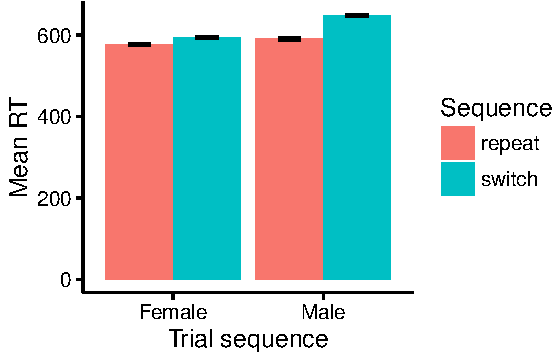
\includegraphics{Lab5_files/figure-latex/unnamed-chunk-2-1}

\begin{Shaded}
\begin{Highlighting}[]
\KeywordTok{ggplot}\NormalTok{(plot_means,}\KeywordTok{aes}\NormalTok{(}\DataTypeTok{x=}\NormalTok{Sequence, }\DataTypeTok{y=}\NormalTok{MeanRT, }\DataTypeTok{group=}\NormalTok{Gender,}\DataTypeTok{shape=}\NormalTok{Gender))+}
\StringTok{  }\KeywordTok{geom_line}\NormalTok{()+}
\StringTok{  }\KeywordTok{geom_point}\NormalTok{()+}
\StringTok{  }\KeywordTok{geom_errorbar}\NormalTok{(limits, }\DataTypeTok{width=}\NormalTok{.}\DecValTok{3}\NormalTok{)+}
\StringTok{  }\KeywordTok{theme_classic}\NormalTok{(}\DataTypeTok{base_size=}\DecValTok{12}\NormalTok{)+}
\StringTok{  }\KeywordTok{ylab}\NormalTok{(}\StringTok{"Mean RT"}\NormalTok{)+}
\StringTok{  }\KeywordTok{xlab}\NormalTok{(}\StringTok{"Trial sequence"}\NormalTok{)}
\end{Highlighting}
\end{Shaded}

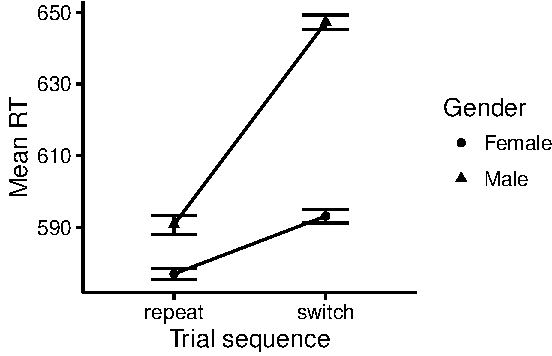
\includegraphics{Lab5_files/figure-latex/unnamed-chunk-3-1}

The graphs show that the switch costs (difference between repeat and
switch trials) is smaller for women and men. Which is good, because we
are simulating the data with this outcome in mind.

\subsection{Running the ANOVA}\label{running-the-anova}

The next step is to conduct an ANOVA. This design has two factors or
independent variables, gender and trial sequence. The gender variable is
between-subjects, and the trial sequence variable is within subjects.
So, we will run a 2 (Gender: Female vs.~Male) x 2 (trial sequence:
Repeat vs.~Switch) mixed design ANOVA with Gender as the betwen-subjects
factor, and trial sequence as the within-subjects factor.

\begin{Shaded}
\begin{Highlighting}[]
\KeywordTok{library}\NormalTok{(broom)}
\NormalTok{all_data$Subject<-}\KeywordTok{as.factor}\NormalTok{(all_data$Subject)}
\NormalTok{aov.out<-}\KeywordTok{aov}\NormalTok{(RT~Gender*Sequence+}\KeywordTok{Error}\NormalTok{(Subject/Sequence),all_data)}
\NormalTok{aov_summary<-}\KeywordTok{summary}\NormalTok{(aov.out)}
\KeywordTok{kable}\NormalTok{(}\KeywordTok{xtable}\NormalTok{(aov_summary),}\DataTypeTok{format=}\StringTok{"latex"}\NormalTok{)}
\end{Highlighting}
\end{Shaded}

\begin{tabular}{l|r|r|r|r|r}
\hline
  & Df & Sum Sq & Mean Sq & F value & Pr(>F)\\
\hline
Gender & 1 & 11458.225 & 11458.2250 & 22.10104 & 1.78e-04\\
\hline
Residuals & 18 & 9332.050 & 518.4472 & NA & NA\\
\hline
Sequence & 1 & 13140.625 & 13140.6250 & 38.47507 & 7.50e-06\\
\hline
Gender:Sequence & 1 & 4060.225 & 4060.2250 & 11.88813 & 2.87e-03\\
\hline
Residuals & 18 & 6147.650 & 341.5361 & NA & NA\\
\hline
\end{tabular}

\begin{Shaded}
\begin{Highlighting}[]
\NormalTok{mt<-}\KeywordTok{model.tables}\NormalTok{(aov.out,}\StringTok{"means"}\NormalTok{)}
\NormalTok{mt}
\end{Highlighting}
\end{Shaded}

\begin{verbatim}
## Tables of means
## Grand mean
##         
## 602.075 
## 
##  Gender 
## Gender
## Female   Male 
##  585.1  619.0 
## 
##  Sequence 
## Sequence
## repeat switch 
##  583.9  620.2 
## 
##  Gender:Sequence 
##         Sequence
## Gender   repeat switch
##   Female 577.1  593.2 
##   Male   590.8  647.2
\end{verbatim}

The above shows the ANOVA table and the means for the main effects and
interaction. We also conduct t.test comparisons to look at the switch
costs separately for men and women.

\begin{Shaded}
\begin{Highlighting}[]
\NormalTok{FemaleT<-}\KeywordTok{t.test}\NormalTok{(RT~Sequence,all_data[all_data$Gender==}\StringTok{"Female"}\NormalTok{,],}\DataTypeTok{paired=}\OtherTok{TRUE}\NormalTok{,}\DataTypeTok{var.equal=}\OtherTok{TRUE}\NormalTok{)}
\NormalTok{MaleT<-}\KeywordTok{t.test}\NormalTok{(RT~Sequence,all_data[all_data$Gender==}\StringTok{"Male"}\NormalTok{,],}\DataTypeTok{paired=}\OtherTok{TRUE}\NormalTok{,}\DataTypeTok{var.equal=}\OtherTok{TRUE}\NormalTok{)}
\NormalTok{FemaleT}
\end{Highlighting}
\end{Shaded}

\begin{verbatim}
## 
##  Paired t-test
## 
## data:  RT by Sequence
## t = -2.3034, df = 9, p-value = 0.04674
## alternative hypothesis: true difference in means is not equal to 0
## 95 percent confidence interval:
##  -31.9115634  -0.2884366
## sample estimates:
## mean of the differences 
##                   -16.1
\end{verbatim}

\begin{Shaded}
\begin{Highlighting}[]
\NormalTok{MaleT}
\end{Highlighting}
\end{Shaded}

\begin{verbatim}
## 
##  Paired t-test
## 
## data:  RT by Sequence
## t = -6.0205, df = 9, p-value =
## 0.0001975
## alternative hypothesis: true difference in means is not equal to 0
## 95 percent confidence interval:
##  -77.59196 -35.20804
## sample estimates:
## mean of the differences 
##                   -56.4
\end{verbatim}

\subsection{Writing up the results}\label{writing-up-the-results}

The next step is to interpret the results and write them up. Here is an
example write-up.

The mean reaction times for each subject in trial sequence condition
were submitted to a 2 (Gender: Female vs.~Male) x 2 (trial sequence:
Repeat vs.~Switch) mixed design ANOVA with Gender as the betwen-subjects
factor, and trial sequence as the within-subjects factor. Mean reaction
times in each condition collapsed across subjects are displayed in
Figure 1.

The main effect of gender was significant, F(1, 18) = 22.1, MSE =
518.45, p \textless{} 0. Women (585 ms) had faster mean reaction times
than men (619 ms).

The main effect of trials sequence was significant, F(1, 18) = 38.48,
MSE = 341.54, p \textless{} 0. Repeat trials (584) had faster mean
reaction times than switch trials (620).

Most important was the significant two-way interaction between gender
and trial sequence, F(1, 18) = 11.89, MSE = 341.54, p \textless{} 0.003.
We interpreted the interaction further by conducting the following
comparisons. Women showed a significant switch cost, t(9) = -2.3, p =
0.047, with faster mean reaction times for repeat (577) than switch
(593) trials. Men also showed a significant switch cost, t(9) = -6.02, p
= 0, with faster mean reaction times for repeat (591) than switch trials
(647). The presence of an interaction indicates that the size of the
switch cost for women was significantly smaller than the size of the
switch cost for men.

